\documentclass[
	a4paper,
	parskip
]{scrartcl}

\usepackage[english]{babel}
\usepackage{authblk}
\usepackage{amsthm}
\usepackage{amsmath}
\usepackage{amssymb}
\usepackage{booktabs}
\usepackage{float}
\usepackage{multirow}
\usepackage{physics}
\usepackage{siunitx}
\usepackage{hyperref}
\usepackage{cleveref}
\usepackage{subcaption}
\usepackage[
  backend=biber,
  sorting=none
]{biblatex}
\usepackage[american]{circuitikz}
\usepackage{glossaries}

\addbibresource{literature.bib}

\makeglossaries
\newglossaryentry{s5990}{name=S5990, description={Hamamatsu two-dimensional PSD}}
\newacronym{psd}{PSD}{position-sensitive detector}

\title{Position-sensitive device}
\author{Bodo Kaiser}
\affil{Ludwig-Maximilians-Universität München}
\affil{\textit{bodo.kaiser@physik.uni-muenchen.de}}

\begin{document}

\maketitle
\tableofcontents

\section{Introduction}

We define a position-sensitive device as a device that outputs voltages proportional to the center of mass coordinates of a light beam incident on a sensitive area.

The present document summarizes the insights acquired on the journey of building such a device.

\subsection{Motivation}

Position-sensitive devices are used in a wide range of industrial and commercial applications, including displacement sensing and beam alignment, see Ref.~\cite[p.~22]{Maekynen00}.

We are interested in using a position-sensitive device for beam pointing alignment in our quantum optics laboratory.

The beam pointing refers to a laser beam's spatial focus and can change through thermal and mechanical effects.
Uncompensated changes in beam alignment can quickly degrade the overall performance of an optical system.
Therefore, it is crucial to align the beam pointing to ensure the optical system's proper operation at hand.

\subsection{Overview}

This document is organized as follows.

The first two sections introduce the theory of the (position-sensitive) photodiode and the operational amplifier.
These sections are rather elaborate and should be skipped by the pragmatic scientist.

The third section describes the (electrical) schematics of the detector.
If you want to adjust parameters, e.g., gain or bandwidth, you should read these sections.

The fourth section is the only significant section if you want to build a \gls{psd}.
If you also want an example of using the \gls{psd} in an optical setup to determine the spatial resolution, you should also read the fifth section.
Finally, the appendix gives some guidance on troubleshooting.

\subsection{Requirements}

The requirements are specified rather loose. The only hard requirement concerns the connectors and voltages of the power supply. The power connector should be a LEMO4 whose pin configuration is compatible with the \SI{\pm15}{\volt} dual-voltage power supplies used in the labs. Features that would be nice to have are:
\begin{enumerate}
	\item The device should be sensible with optical powers that are safe to operate, i.e., $P<\SI{1}{\micro\watt}$. There is no preferred wavelength.
	\item For easy integration into existing optical setups, the device should be as compact as possible. Additional space, if needed, should be occupied by elonging the height. The sensitive area of the detector should be on the bottom. The connectors should be on the top to avoid cables blocking the beam path.
	\item It should be possible to mount different detector sizes on the device.
\end{enumerate}
The range of the output voltages of the device can be chosen for the optimal signal-to-noise ratio.

\subsection{Specification}

\begin{figure}[H]
	\centering
	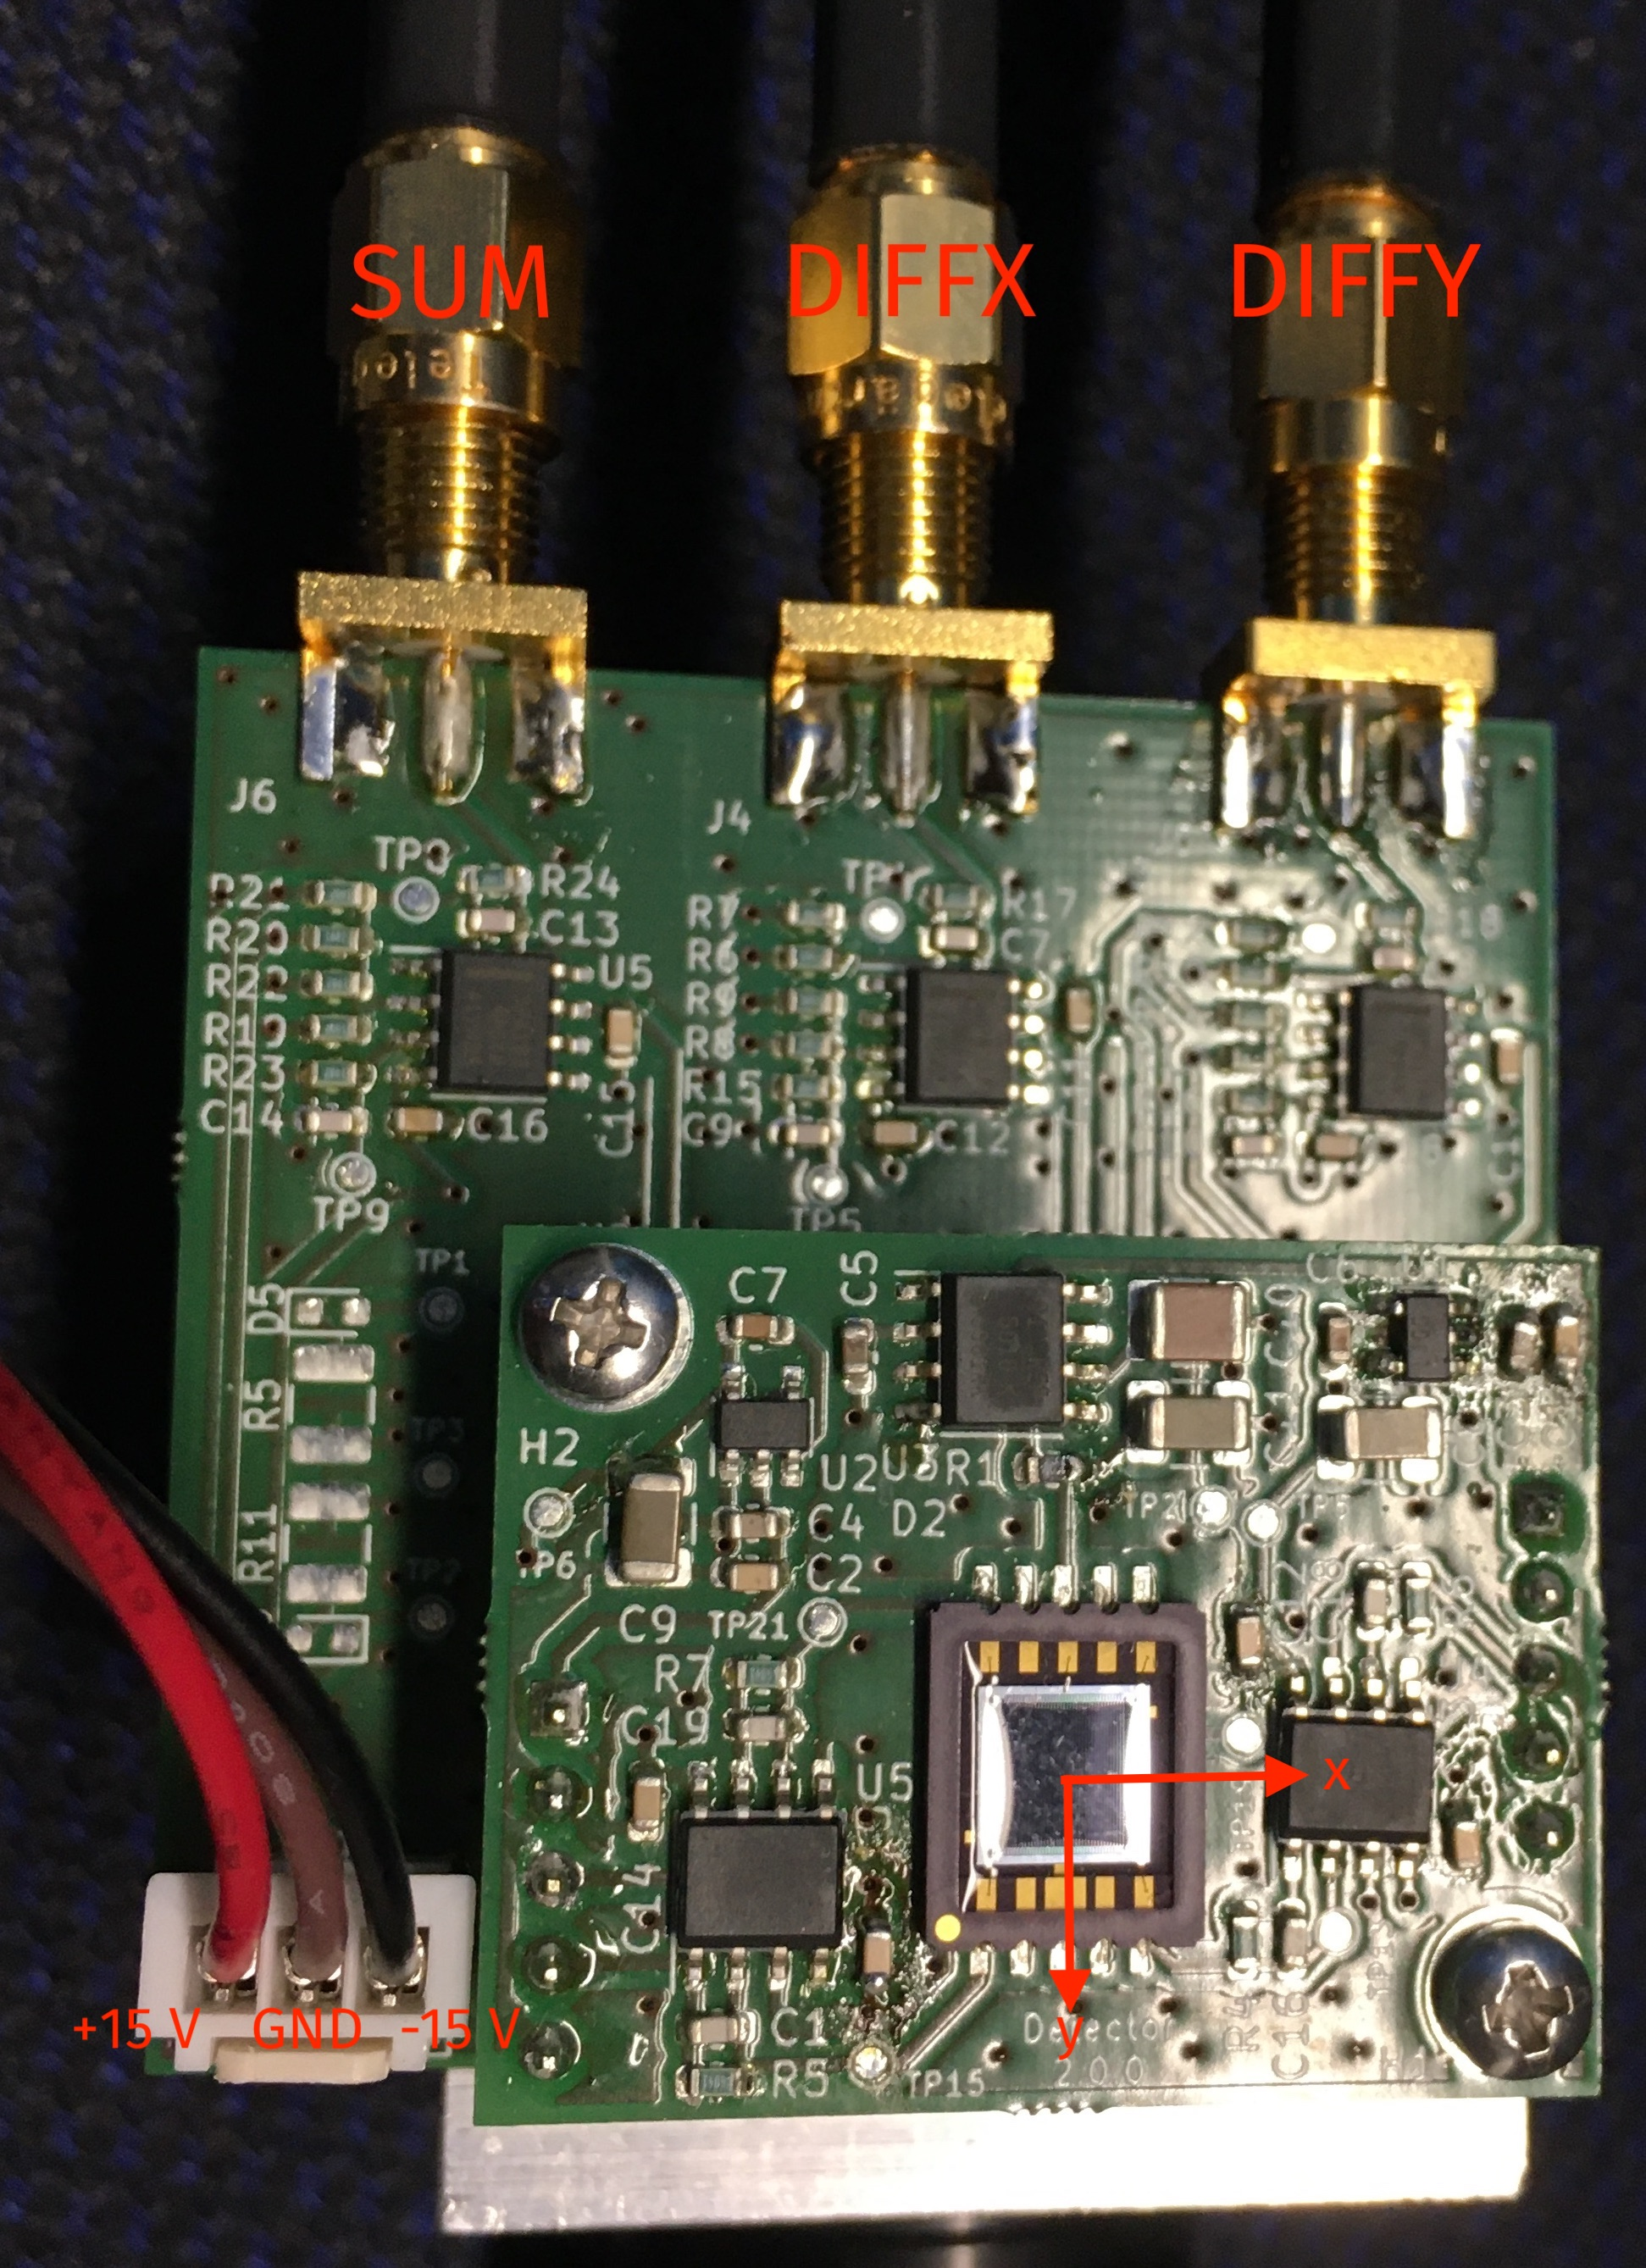
\includegraphics[scale=0.2]{detector.jpg}
	\caption{\gls{psd} on optical mount with connected cables}\label{fig:detector}
\end{figure}
\Cref{fig:detector} shows an image of the \gls{psd}.
The output voltage signals can be tapped from the upper \gls{sma} connectors.
The upper left connector gives the SUM voltage which reflects the total intensity of the optical signal.
The upper center connector gives the DIFFX voltage which reflects the difference proportional to the horizontal position on the sensitive area.
The upper right connector gives the DIFFY voltage which is proportional to the vertical position.
The SUM voltage is required to normalize the difference signals.
The DIFFX voltage increases when moving the light beam on the sensitive area to the right while the DIFFY voltage increases while moving the light beam to the bottom.
The device is powered by a 3-pin connector.
The outer (left) cable is the positive \SI{+15}{\volt} supply while the opposite cable is negative \SI{-15}{\volt} supply.
The center cable of the 3-pin connector has to reference ground.
The power connector has no polarity protection so be careful!

\begin{table}[htb]
  \centering
  \begin{tabular}{lcccc}
    \toprule
      Parameter & Minimum & Typical & Maximum \\
    \midrule
      Output voltages & \SI{-13}{\volt} & \SIrange{-2}{+2}{\volt} & \SI{+13}{\volt} \\
      Supply voltages & \SI{\pm13}{\volt} & \SI{\pm15}{\volt} & \SI{\pm37}{\volt} \\
      Spatial resolution & \SI{5.0}{\micro\meter} & \SI{2}{\micro\meter} & \SI{1}{\micro\meter} \\
      Bandwidth & & \SI{1400}{\kilo\hertz} & \\
    \bottomrule
  \end{tabular}
  \captionsetup{width=.8\textwidth}
  \caption{Specifications of the presented \gls{psd}}\label{tab:specifications}
\end{table}
\Cref{tab:specifications} summarizes the specifications of the presented \gls{psd}.
These specifications are only a rough estimate and we only assembled one \gls{psd} so far.
\section{Position-sensitive detector}

% TODO: overview of position-sensitive detectors and why we choose the lateral pin-cushion type

% TODO: specify pages \cite{Noorlag74}

% TODO: diagram of depletion region for lateral photodiode
% TODO: motivate value for reverse bias
% TODO: diode leakage current
% TODO: noise model
% TODO: responsitivity
% TODO: bandwidth limit
% TODO: photon shot noise

\begin{figure}[H]
	\centering
	\begin{circuitikz}
		\draw (0, 0) node[circ]{};
		\draw (+2, +2) node[ocirc, label=X1]{} to[photodiode] (0, 0);
		\draw (-2, -2) node[ocirc, label=X2]{} to[photodiode] (0, 0);
		\draw (+2, -2) node[ocirc, label=Y2]{} to[photodiode] (0, 0);
		\draw (-2, +2) node[ocirc, label=Y1]{} to[photodiode] (0, 0);
		\draw (0, 0) -- ++(0, -2.5) node[ocirc, label=Cathode, rotate=180]{};
	\end{circuitikz}
	\caption{Position-sensitive detector as photodiodes}
\end{figure}

% TODO: mention non-linearity of voltage response to illumination

\begin{figure}[H]
	\centering
	\begin{circuitikz}
		\draw (-3, -2) to[current source, l=$I_\text{photo}$] ++(0, 4);
		\draw (-1, -2) node[circ]{} to[current source, l=$I_\text{dark}$] ++(0, 4) node[circ]{};
		\draw (1, -2) node[circ]{} to[resistor, l=$R_d$] ++(0, 4) node[circ]{};
		\draw (3, -2) to[capacitor, l=$C_d$] ++(0, 4);
		\draw (-3, -2) -- ++(6, 0);
		\draw (-3, 2) -- ++(6, 0);
		\draw (0, -2) -- ++(0, -1) node[ocirc, label=Cathode, rotate=180]{};
		\draw (0, 2) -- ++(0, 1) node[ocirc, label=Anode]{};
	\end{circuitikz}
	\caption{Photodiode equivalent circuit}
\end{figure}

\begin{equation}
	I_\text{leakage}=I_\text{dark}\left(1-e^{\frac{qV_d}{k_BT}}\right)
\end{equation}
\section{Preamplifier}

The photocurrents created by our detector are in the range of microampere where they are vulnerable to noise.
Using a preamplifier, we can increase the amplitude of the signal for an improved signal-to-noise ratio.
The typical photocurrent preamplifier is based on the transimpedance (current-to-voltage) amplifier design using a voltage-feedback operational amplifier.
Converting the current to a voltage signal has the benefit that the voltage signal can be easily visualized with an oscilloscope.
Furthermore, the voltage-feedback operational amplifier design appears to be more common than the current-feedback operational amplifier, as manufacturers offer much more choice and they are more prominent in the literature.
That said, current feedback operational amplifiers are reported to be a viable solution for high-speed and high-bandwidth applications, see Ref.~\cite[p.~110]{Jung05} for an overview of the benefits of current feedback amplifiers and Ref.~\cite[Ch.~9]{Carter17} for a comparison.

% TODO: mention feedback tee network for high feedback factor
% TODO: mention finite loop gain error (Jung, p. 13)
% TODO: table with op amp parameters specified in the datasheet and their relevance for our application
% TODO: noise model (Jung, p. 80)

\subsection{Gain}

\begin{figure}[H]
	\centering
	\begin{circuitikz}
		\draw (0, 0) node[op amp](opamp){};
		\draw (opamp.+) -- +(0, -1) node[ground](gnd1){};
		\draw (opamp.out) -- (3, 0) node[ocirc, label=$V_\text{out}$]{};
		\draw (opamp.-) to[current source, invert, l=$I_\text{in}$] +(-3, 0) node(node1){} -- (node1 |- gnd1) node[ground]{};
		\draw (opamp.-) |- (-1, 2) to[resistor, l=$R_f$] (1,2) -| (opamp.out);
	\end{circuitikz}
	\caption{Simple transimpedance amplifier circuit.}
\end{figure}

\begin{equation}
	V_\text{out}=R_fI_\text{in}
\end{equation}

\begin{figure}[H]
	\begin{subfigure}[t]{.5\textwidth}
		\centering
		\begin{circuitikz}
			\draw (0, 0) node[op amp](opamp){};
			\draw (opamp.+) -- +(0, -1) node[ground](gnd1){};
			\draw (opamp.out) -- +(.5, 0) node[ocirc, label=$V_\text{out}$]{};
			\draw (opamp.-) -- +(-3, 0) node(node1){} to[current source, invert, l=$I_\text{in}$] (node1 |- gnd1) node[ground]{};
			\draw (node1) -- +(1.5, 0) node(node2){} to[resistor, l=$R_\text{in}$] (node2 |- gnd1) node[ground]{};
			\draw (opamp.-) |- (-1, 2) to[resistor, l=$R_f$] (1,2) -| (opamp.out);
		\end{circuitikz}
		\caption{Transimpedance amplifier.}
	\end{subfigure}
	\begin{subfigure}[t]{.5\textwidth}
		\centering
		\begin{circuitikz}
			\draw (0, 0) node[op amp](opamp){};
			\draw (opamp.+) -- +(0, -1) node[ground](gnd1){};
			\draw (opamp.out) -- +(.5, 0) node[ocirc, label=$V_\text{out}$]{};
			\draw (opamp.-) to[resistor, l_=$R_\text{in}$] +(-3, 0) node(node1){} to[voltage source, l=$V_\text{in}{=}R_\text{in}I_\text{in}$] (node1 |- gnd1) node[ground]{};
			\draw (opamp.-) |- (-1, 2) to[resistor, l=$R_f$] (1,2) -| (opamp.out);
		\end{circuitikz}
		\caption{Inverting amplifier.}
	\end{subfigure}
	\caption{Equivalence between transimpedance and inverting amplifier using source transformation.}
\end{figure}

\subsection{Offset}

\subsubsection{Input offset voltage}

\cite[p.~54]{Jung05}

\begin{figure}[H]
	\centering
	\begin{circuitikz}
		\draw (0, 0) node[op amp](opamp){};
		\draw (opamp.out) -- +(.5, 0) node[ocirc, label=$V_\text{out}$]{};
		\draw (opamp.-) to[resistor, l_=$R_\text{in}$] +(-3, 0) node(node1){} to[voltage source, l=$V_\text{in}$] (node1 |- +0, -3) node[ground](gnd){};
		\draw (opamp.-) |- (-1, 2) to[resistor, l=$R_f$] (1,2) -| (opamp.out);
		\draw (opamp.+) -- ++(0, -1) node(node2)[circ]{};
		\draw (-2, -0.5) to[potentiometer, n=pot, l_=$R_p$] (-2, -2.5);
		\draw (node2) -- ++(2, 0) node(node3){} to[resistor, l_=$R_c$] (node3 |- gnd) node[ground]{};
		\draw (node2) -- (pot.wiper);
		\draw (-2, -0.5) node[ocirc, label=$+V_s$]{};
		\draw (-2, -2.5) node[ocirc, label=$-V_s$, rotate=180]{};
	\end{circuitikz}
	\caption{Input current offset compensation.}
\end{figure}

\subsubsection{Input bias current}

% TODO: mention that I+, I- are difficult to measure and therefore the datasheets report Ibias and Ioffset

\begin{figure}[H]
	\begin{subfigure}[t]{.5\textwidth}
		\centering
		\begin{circuitikz}
			\draw (0, 0) node[op amp, scale=1.2](opamp){};
			\draw (opamp.out) -- +(0.5, 0) node[ocirc, label=$V_\text{out}$]{};
			\draw (opamp.+) -- +(-0.5, 0) node(node1a)[circ]{} to[current source, l=$I_\text{offset}/2$] (node1a |- opamp.-) node(node1b)[circ]{} -- (opamp.-);
			\draw (node1a) -- ++(-1, 0) node(node2a)[circ]{} -- ++(0, -0.5) to[current source, l=$I_\text{bias}$] ++(0, -1) node[ground]{};
			\draw (node1b) -- ++(-1, 0) node(node2b)[circ]{} -- ++(0, +0.5) to[current source, l_=$I_\text{bias}$] ++(0, 1) node[ground, rotate=180]{};
			\draw (node2a) to[short, i<=$i_+$] +(-1.5, 0) node[ocirc, label=$V_+$]{};
			\draw (node2b) to[short, i<_=$i_-$] +(-1.5, 0) node[ocirc, label=$V_-$]{};
		\end{circuitikz}
		\caption{Equivalent current sources as reported in the datasheet.}
	\end{subfigure}
	\begin{subfigure}[t]{.5\textwidth}
		\centering
		\begin{circuitikz}
			\draw (0, 0) node[op amp, scale=1.2](opamp){};
			\draw (opamp.out) -- +(0.5, 0) node[ocirc, label=$V_\text{out}$]{};
			\draw (opamp.+)-- ++(-0.5, 0) node(node2a)[circ]{} -- ++(0, -0.5) to[current source, l=$I_-$] ++(0, -1) node[ground]{};
			\draw (opamp.-) -- ++(-0.5, 0) node(node2b)[circ]{} -- ++(0, +0.5) to[current source, l_=$I_+$] ++(0, 1) node[ground, rotate=180]{};
			\draw (node2a) to[short, i<=$i_+$] +(-1.5, 0) node[ocirc, label=$V_+$]{};
			\draw (node2b) to[short, i<_=$i_-$] +(-1.5, 0) node[ocirc, label=$V_-$]{};
		\end{circuitikz}
		\caption{Alternative equivalent current sources.}
	\end{subfigure}
	\caption{Non-zero input current from the operational amplifier.}
\end{figure}

\begin{align}
	I_+=I_\text{bias}+\frac{1}{2}I_\text{offset} &&
	I_\text{offset}=I_+-I_- \\
	I_-=I_\text{bias}-\frac{1}{2}I_\text{offset} &&
	I_\text{bias}=\frac{I_++I_-}{2}
\end{align}

\begin{figure}[H]
	\centering
	\begin{circuitikz}
		\draw (0, 0) node[op amp](opamp){};
		\draw (opamp.out) -- +(.5, 0) node[ocirc, label=$V_\text{out}$]{};
		\draw (opamp.-) to[resistor, l_=$R_\text{in}$] +(-3, 0) node(node1){} to[voltage source, l=$V_\text{in}$] (node1 |- +0, -3) node[ground](gnd){};
		\draw (opamp.-) |- (-1, 2) to[resistor, l=$R_f$] (1,2) -| (opamp.out);
		\draw (opamp.+) -- ++(0, -1) node(node2)[circ]{} to[resistor, l_=$R_c$] (opamp.+ |- gnd) node[ground]{};
		\draw (node2) -- ++(1, 0) node(node3){} to[capacitor, l=$C_c$] (node3 |- gnd) node[ground]{};
	\end{circuitikz}
	\caption{Input current offset compensation.}
\end{figure}

\cite[p.~57]{Jung05}
\cite[p.~25]{Graeme96}

\begin{equation}
	R_c=\frac{R_\text{in}R_f}{R_\text{in}+R_f}
\end{equation}

% TODO: mention that this only works for well-matched bias currents (Ioffset < Ibias)
% TODO: give noise argument why this introduces more error

\subsection{Noise}

\subsection{Stability}

\cite[p.~693]{Hobbs11}
\cite[p.~183]{Kay12}
\cite[Ch.~5]{Carter17}
\cite[Ch.~3]{Graeme96}

% TODO: pcb design
% TODO: power management

\printglossaries
\printbibliography

\end{document}